\chapter{Описание практической части}
\label{cha:ch_5}

\section{Симуляции и первый образец модели}

При подготовке к созданию итоговой модели в первую очередь создавались симуляции (искуственные 
данные, похожие по статистическим распределениям на настоящие, но по своей структуре более простые). \\

После этого на созданных симуляциями данных тренировались первые образцы нейросетевых моделей. 
Общая архитектура схожа с моделью из статьи \cite{Bonjean}, но в данном случае вместо слоёв Dropout 
использовались слои батч-нормализации и вместо 5 блоков было добавлено 3 блока с 32 фильтрами в 
первом блоке. \\

\begin{figure}
	\begin{minipage}[h]{0.32\linewidth}
		\center{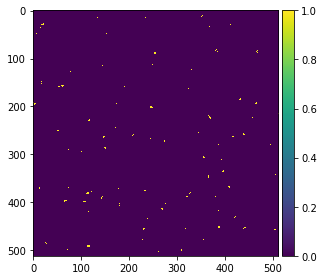
\includegraphics[width=\linewidth]{sym0}\\a)}
	\end{minipage}
	\begin{minipage}[h]{0.32\linewidth}
		\center{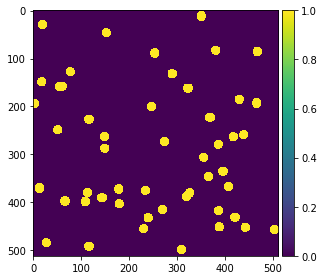
\includegraphics[width=\linewidth]{sym1}\\b)}
	\end{minipage}
	\begin{minipage}[h]{0.32\linewidth}
		\center{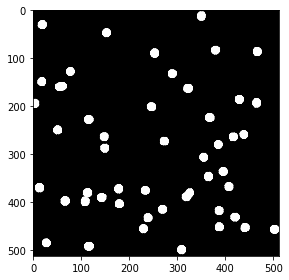
\includegraphics[width=0.9\linewidth]{sym2}\\c)}
	\end{minipage}

	\caption{a) Данные объектов из симуляций; b) Данные источников из симуляций; 
		c) Результат работы нейросети;}
\end{figure}

Выше приведен пример работы симуляции а также пример сегментированного изображения. Итоговая точность 
сегментации составляет 0.9978 для симулированных данных.\\

\section{Обработка каталога скоплений}

Далее, начинается обработка настоящих данных. Нужно загрузить и обработать каталог скоплений Planck, 
который будет разделен на два подкаталога: 
\begin{enumerate}
	\item planck\_z (скопления с измеренным красным сдвигом)
	\item planck\_no\_z (скопления без информации о красном сдвиге)
\end{enumerate}

\section{Обработка данных PS1}

Поскольку поиск в базе данных PS1 можно вести только в системе координат ICRS, центры скоплений 
нужно преобразовать в нужный вид. Однако проекция healpix будет использовать галактические 
координаты, поэтому координаты найденных объектов будут сохранены соответственно в галактической 
системе.\\

После того, как были получены данные по скоплениям, можно начать загрузку и обработку данных из 
обзоров PS1. В каждом пикселе из разбиения с $n_{side}=2$ генеруется определенное количество патчей. 
Центры патчей выбираются случайным образом как пиксели, рядом с которыми есть скопления. Размер каждого 
патча задан как 2048 x 2048 в разбиении с $n_{side}=2^{17}$, и так как пиксели HEALPix могут иметь 
протяжённую структуру, итоговый радиус патча вычислялся как расстояние от центра патча до дальнего 
угла для патча размером 2050 x 2050. В итоге максимальный радиус оказался равен 
$\approx 0.9^{\circ}$. Для преобразований использовалась библиотека healpy.\\

\begin{figure}[ht]
	\begin{minipage}[h]{0.44\linewidth}
		\center{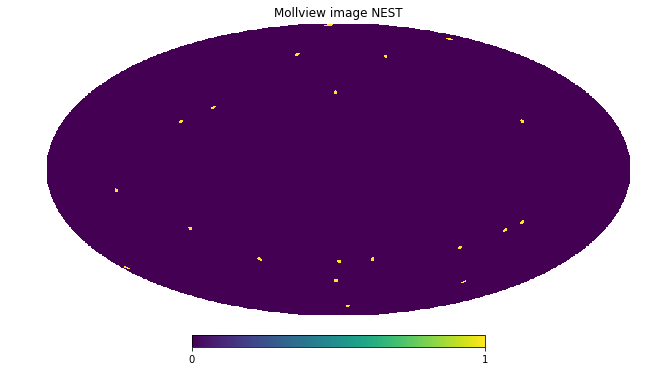
\includegraphics[width=\linewidth]{patch0}\\a)}
	\end{minipage}
	\begin{minipage}[h]{0.44\linewidth}
		\center{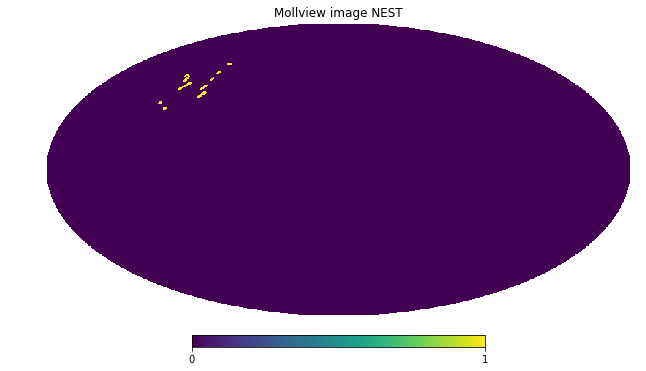
\includegraphics[width=\linewidth]{patch1}\\b)}
	\end{minipage}

	\caption{Сгенерированные центры патчей: a) Для всего неба; 
b) Для пикселя №6 из разбиения $n_{side}=2$;}
\end{figure}

Далее данные нужно преобразовать в формат двумерных матриц для загрузки в нейросеть, перед этим 
вычислив для каждого объекта номер пикселя healpix, к которому он относится. Объекты, относящиеся 
к одним и тем же пикселям, нужно соответствующим образом отождествить, сохранив те, для которых 
значения ошибок меньше.\\

\begin{figure}[ht]
	\center{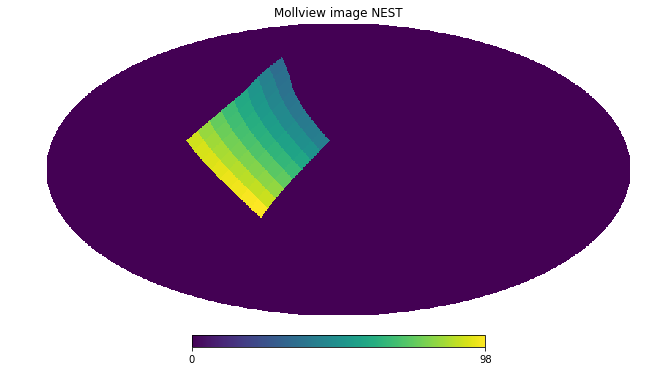
\includegraphics[width=0.8\linewidth]{pix2pic0}}
	\caption{Пример расположения двумерной матрицы на проекции неба для большего разбиения HEALPix}
\end{figure}

Для этого создавались матрицы соответсвий между координатами изображения и номерами пикселей из 
healpix-разбиения. Перед началом создания такой матрицы мы всегда знаем номер пикселя для центра 
изображения, в нашем случае для координат $(1023, 1023)$. Библиотека healpy позволяет находить 8
соседних пикселей, зная вектор координат для заданного пикселя, поэтому постепенно, начиная с центра,
можно найти все пиксели изображения.\\

После этого по построенным матрицам нужно каждый объект перенести на изображение.
Это можно сделать двумя способами:

\begin{itemize}
	\item Для яркости объекта можно на изображение на полученные координаты нанести круг с 
		радиусом, пропорциональным яркости. Тогда матрица будет состоять из нулей и единиц. Такой 
		метод подходит для визуальной оценки правильности преобразования координат.
	\item В заданные координаты записать значение нужного параметра. Такие матрицы и будут 
		отправлены в нейросеть на обучение. Состоят из значений с плавающей точкой.
\end{itemize}

Точно так же перенести на двумерное изображение нужно и маски, определяющие наличие скоплений в 
данной области. Для каждого скопления вычисляются номера пикселей в радиусе $5'$, после чего они с 
помощью той же матрицы соответствий переносятся на изображение.\\
